%&pdfLaTeX
% !TEX encoding = UTF-8 Unicode
\documentclass{article}
\usepackage{ifxetex}
\ifxetex
\usepackage{fontspec}
\setmainfont[Mapping=tex-text]{STIXGeneral}
\else
\usepackage[T1]{fontenc}
\usepackage[utf8]{inputenc}
\fi
\usepackage{textcomp}

\usepackage{tabularx}
\usepackage{graphicx}
\usepackage{ulem}
\usepackage{amssymb}
\usepackage{fancyhdr}
\usepackage{float}
\usepackage{url}
\usepackage[colorlinks=true,
            linkcolor=red,
            urlcolor=blue,
            citecolor=gray]{hyperref}
\newcommand{\ttilde}[0]{\raise.17ex\hbox{$\scriptstyle\sim$}}
\renewcommand{\vec}[1]{\ensuremath{\mathbf{#1}}}
\newcommand{\evec}[1]{\ensuremath{\mathbf{\hat #1}}}

\renewcommand{\headrulewidth}{0pt}
\renewcommand{\footrulewidth}{0pt}
\usepackage{color}
\usepackage[a4paper,vmargin={20mm,20mm},hmargin={20mm,10mm}]{geometry}
% \usepackage{listings}
% \lstset{inputencoding=ansinew}

\definecolor{color18}{rgb}{0.07,0.33,0.80}

\setlength\parindent{0pt}

\usepackage{times}
\usepackage{textpos}

\begin{document}

%%%%%%%%%%%%%%%%%%%%%%%%%%%%%%
%%% START OF CIG MANUAL COVER TEMPLATE %%%
%%%%%%%%%%%%%%%%%%%%%%%%%%%%%%
% This should be pasted at the start of manuals and appropriate strings entered at locations indicated with FILL.
% Be sure the TeX file includes the following packages.
% \usepackage{graphicx}
% \usepackage{times}
% \usepackage{textpos}

\definecolor{dark_grey}{gray}{0.3}

%LINE 1%
{
\renewcommand{\familydefault}{\sfdefault}

\pagenumbering{gobble}
\begin{center}
\resizebox{\textwidth}{!}{\textcolor{dark_grey}{\fontfamily{\sfdefault}\selectfont
COMPUTATIONAL INFRASTRUCTURE FOR GEODYNAMICS (CIG)
}}

\hrule

%LINE 2%
\color{dark_grey}
\rule{\textwidth}{2pt}

%LINE 3%
\color{dark_grey}
% FILL: additional organizations
% e.g.: {\Large Organization 1\\Organization 2}
{\Large }
\end{center}

%COLOR AND CODENAME BLOCK%
\begin{center}
\resizebox{\textwidth}{!}{\colorbox
% FILL: color of code name text box
% e.g. blue
{blue}{\fontfamily{\rmdefault}\selectfont \textcolor{white} {
% FILL: name of the code
% e.g. PyLith
% You may want to add \hspace to both sides of the codename to better center it, such as:
% \newcommand{\codename}{\hspace{0.1in}CodeName\hspace{0.1in}}
\hspace{0.1in}AxiSEM\hspace{0.1in}
}}}
\end{center}

%MAIN PICTURE%
\begin{textblock*}{0in}(0.7in,0.2in)
% FILL: image height
% e.g. height=6.5in
\begin{center}
\vspace{.5in}
\includegraphics[height=5.5in]
% FILL: image file name
% e.g. cover_image.png
{Axisem2png.png}
\end{center}
\end{textblock*}

%USER MANUAL%
\color{dark_grey}
\hfill{\Huge \fontfamily{\sfdefault}\selectfont User Manual \\
% FILL: manual version
% e.g. 1.0
\raggedleft \huge \fontfamily{\sfdefault}\selectfont Version {1.2}\\}

%AUTHOR(S) & WEBSITE%
\null
\vfill
\color{dark_grey}
\Large \hfill {\raggedleft \fontfamily{\sfdefault}\selectfont
% FILL: author list
% e.g. Author One\\Author Two\\Author Three\\
% be sure to have a newline (\\) after the final author
Tarje Nissen-Meyer\\Martin van Driel\\Simon St\"{a}hler\\Kasra Hosseini\\Stefanie Hempel\\Alexandre Fournier\\
}
{\fontfamily{\sfdefault}\selectfont www.geodynamics.org}

\hrule

%LINE%
\color{dark_grey}
\rule{\textwidth}{2pt}

}

\pagebreak
\pagenumbering{arabic}

%%%%%%%%%%%%%%%%%%%%%%%%%%%%%%
%%%   END OF CIG MANUAL COVER TEMPLATE    %%%
%%%%%%%%%%%%%%%%%%%%%%%%%%%%%%

\begin{center}
    \begin{tabularx}{\textwidth}{lX}
        \begin{minipage}{0.3\textwidth}
            \begin{center}
                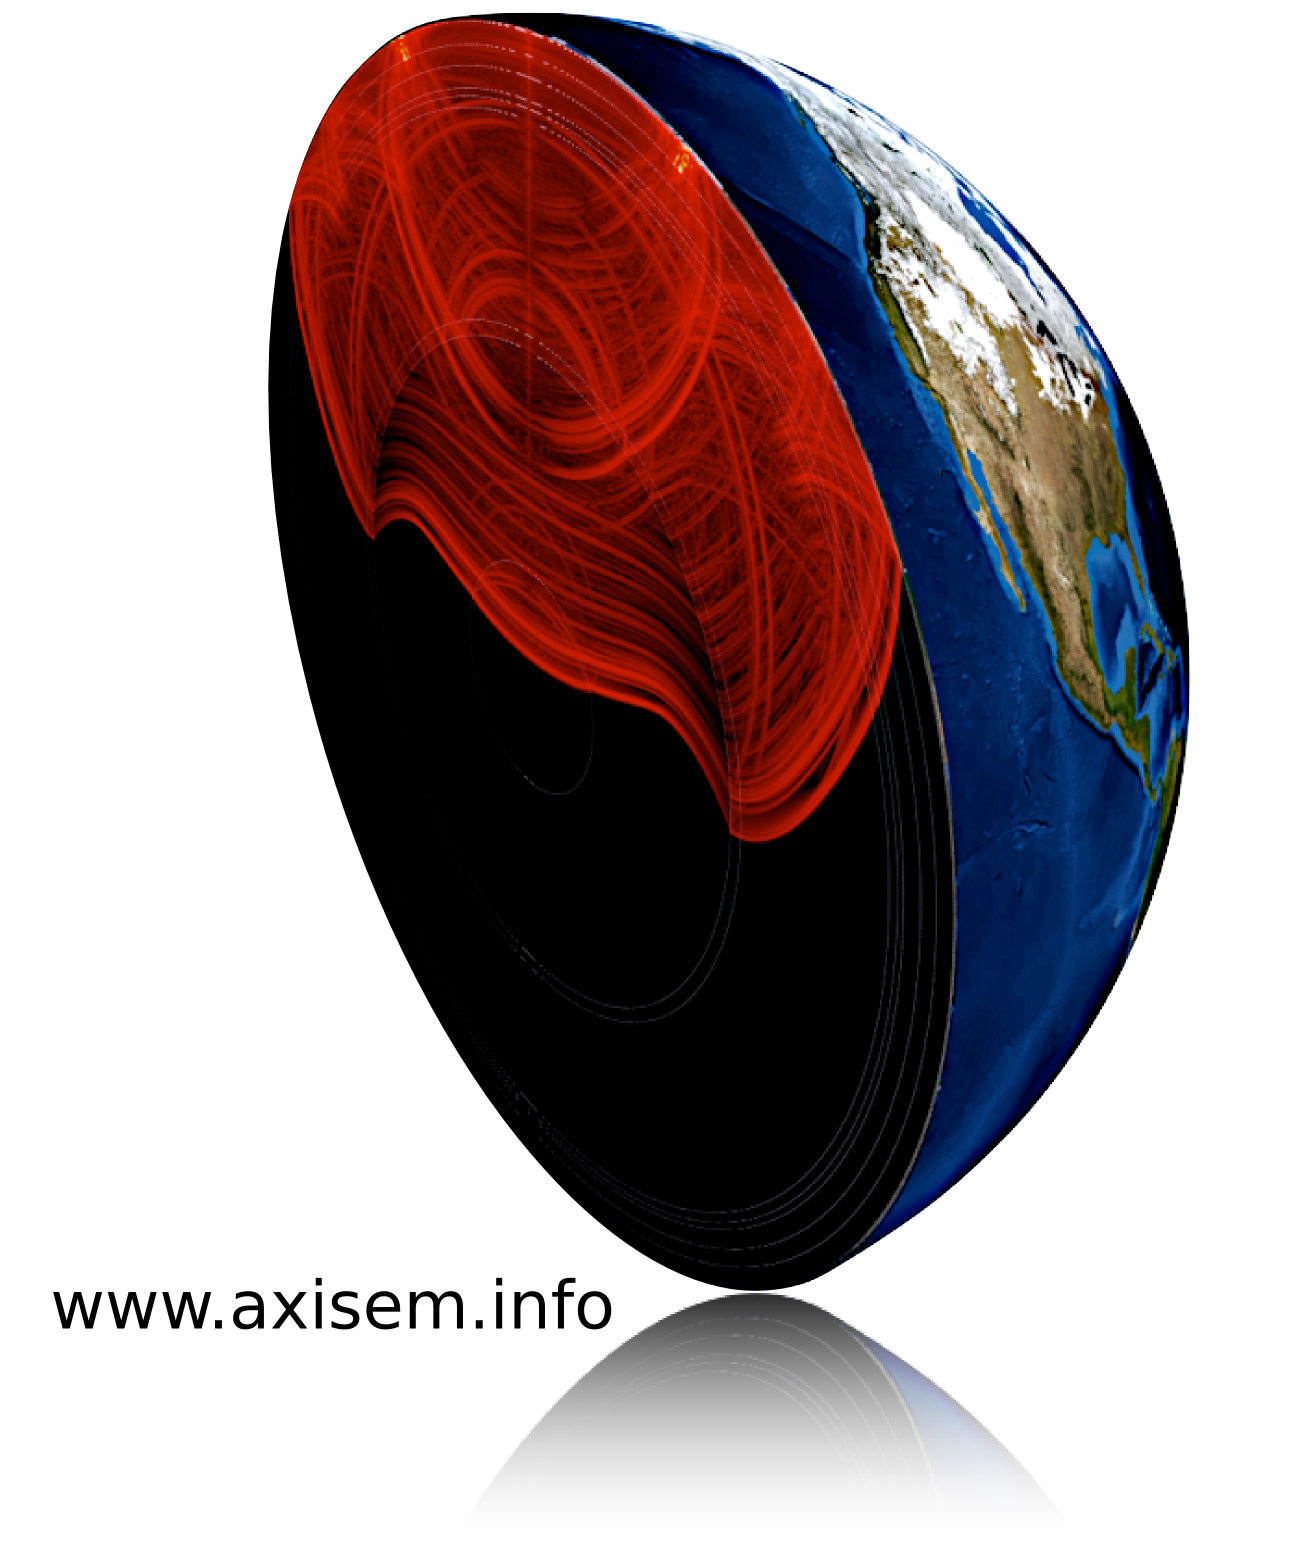
\includegraphics[width=\textwidth]{Axisem2png.png}
            \end{center}
        \end{minipage}
        &
        \begin{minipage}{0.6\textwidth}
            \begin{center}
                \title{}
                \LARGE{ \textbf{\sc AxiSEMv1.2 Manual}}
                \vspace*{0.6cm}\\
                {\large
                Tarje Nissen-Meyer\textsuperscript{1},
                Martin van Driel\textsuperscript{2},
                Simon St\"{a}hler\textsuperscript{3},
                Kasra Hosseini\textsuperscript{3},
                Stefanie Hempel\textsuperscript{4},
                Alexandre Fournier\textsuperscript{5}}
                \vspace*{0.3cm}\\
                {\small  \textsuperscript{1} Oxford University (UK),
                  \textsuperscript{2} ETH Zurich (Switzerland),  \textsuperscript{3}
                  LMU M\"{u}nchen (Germany), \textsuperscript{4} Universit\"{a}t
                  M\"{u}nster (Germany), \textsuperscript{5} IPG Paris
                  (France)}\\
                {\large Oxford, UK -- July 7, 2014}
            \end{center}
        \end{minipage}
    \end{tabularx}
\end{center}

%
%
\noindent {AxiSEM} is a \textbf{parallel spectral-element method} to solve
3D wave propagation in a sphere with axisymmetric or spherically symmetric
visco-elastic, acoustic, anisotropic structures. Such media allow the
computational domain to be collapsed to a 2D disk, where the third, azimuthal
dimension is solved analytically on-the-fly posteriori. This leads to extreme
speedup by many orders of magnitude with respect to methods that discretize the
3D domain, and enables a full coverage of the seismic body- and surface wave
frequency spectrum between 0.001-1Hz.  The time-domain code delivers full
spatio-temporal wavefields that can be stored on disk and transformed to
frequency domain. Due to the dimensional reduction, global wave propagation at
typical seismic of \textbf{periods down to 5 seconds can be tackled on
laptops}, and at 1Hz on moderate clusters.

The Fortran 90 code is divided into a \textbf{Mesher}, a \textbf{Solver}
utilizing the message-passing interface (MPI) for communication between
separate domains, and comprehensive \textbf{post processing} for ease of
visualization.
The essential raison-d'\^{e}tre of this method is the efficient
calculation of seismograms, wavefield movies, and those wavefields that underly
sensitivity kernels to allow for tomographic inversions of any portion of a
seismogram at any relevant frequency.

\begin{center}
\textbf{Portal for this code:} \href{http://www.axisem.info}{www.axisem.info}\\
\textbf{Contact:} \href{mailto:info@axisem.info}{info@axisem.info}
\end{center}

%
\noindent \textbf{Principal authors:} \\
Tarje Nissen-Meyer, Alexandre
Fournier, Martin van Driel, Simon St\"{a}hler, Kasra Hosseini, Stefanie Hempel.\vspace*{0.3cm}\\
\noindent \textbf{Contributions:}\\
 J.-P. Ampuero, E. Chaljub, A. Colombi, F. A. Dahlen, D. Komatitsch,
 G. Nolet, J. Tromp.\vspace*{0.3cm}\\
\noindent \textbf{Research funding:} \\Princeton University, NSF, HP2C Petaquake,
QUEST ITN (Marie Curie), ETH Zurich, Oxford University.\vspace*{0.3cm}\\
%
\noindent \textbf{Copyright}\\
\copyright  \hspace*{0.1cm}
2013, Tarje Nissen-Meyer,
Alexandre Fournier, Martin van Driel, Simon St\"{a}hler, Kasra Hosseini, Stefanie Hempel.\vspace*{0.3cm}\\

AxiSEM is free software: you may redistribute it and/or modify it
under the terms of the GNU General Public License as published by the
Free Software Foundation, either version 3 of the License, or any
later version.

AxiSEM is distributed in the hope that it will be useful, but WITHOUT
ANY WARRANTY; without even the implied warranty of MERCHANTABILITY or
FITNESS FOR A PARTICULAR PURPOSE. Commercial use must be discussed
with the authors prior to usage. See the GNU General Public License
for more details: \verb|LICENSE_GPL.txt|
\newpage
\tableofcontents
%
\vspace*{1cm}

\section{Preliminaries}

\subsection{The AxiSEM Concept}

The basic idea behind AxiSEM is to take advantage of axial symmetry with respect
to an axis going through the center of the earth and the source. In such axisymmetric
models, the response to a moment tensor or single force point source can be expanded in a
series of multipoles (mono-, di- and quadrupole). The dependence of the 3D wavefield on
azimuth $\phi$ can be solved analytically and the remaining 2D problems (four of them for
a full moment tensor source) are solved numerically using a spectral
element approach.\\

\begin{center}
    \begin{minipage}[t]{0.4\paperwidth}
        Source Decomposition:\\
        \begin{minipage}[c]{0.1\paperwidth}
            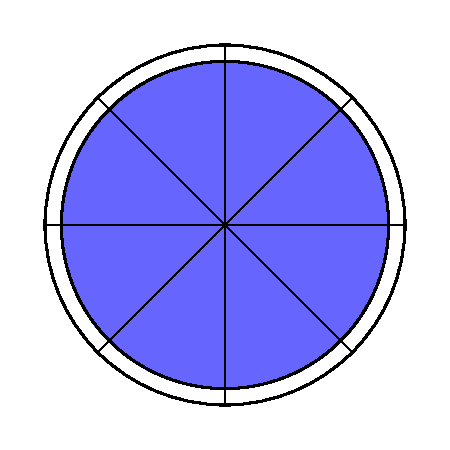
\includegraphics[width=\textwidth]{radpat_mono.pdf}%
        \end{minipage}%
        \begin{minipage}[c]{0.4\paperwidth}
            $\scriptsize{\vec u = \vec u (s,z)}$ \\
        \end{minipage}

        \begin{minipage}[c]{0.1\paperwidth}
            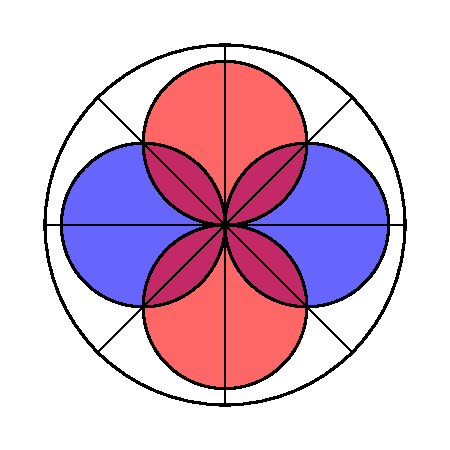
\includegraphics[width=\textwidth]{radpat_di.pdf}
        \end{minipage}%
        \begin{minipage}[c]{0.4\paperwidth}
            $\scriptsize{\vec u = \vec u (s,z)} \cdot f(\sin\phi, \cos\phi)$ \\
        \end{minipage}

        \begin{minipage}[c]{0.1\paperwidth}
            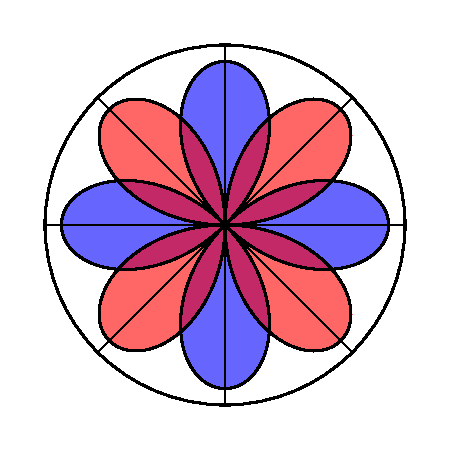
\includegraphics[width=\textwidth]{radpat_quad.pdf}
        \end{minipage}%
        \begin{minipage}[c]{0.4\paperwidth}
            $\scriptsize{\vec u = \vec u (s,z)} \cdot f(\sin(2\phi), \cos(2\phi))$ \\
        \end{minipage}%
    \end{minipage}%
    \begin{minipage}[t]{0.25\paperwidth}
        2D numerical problems:

        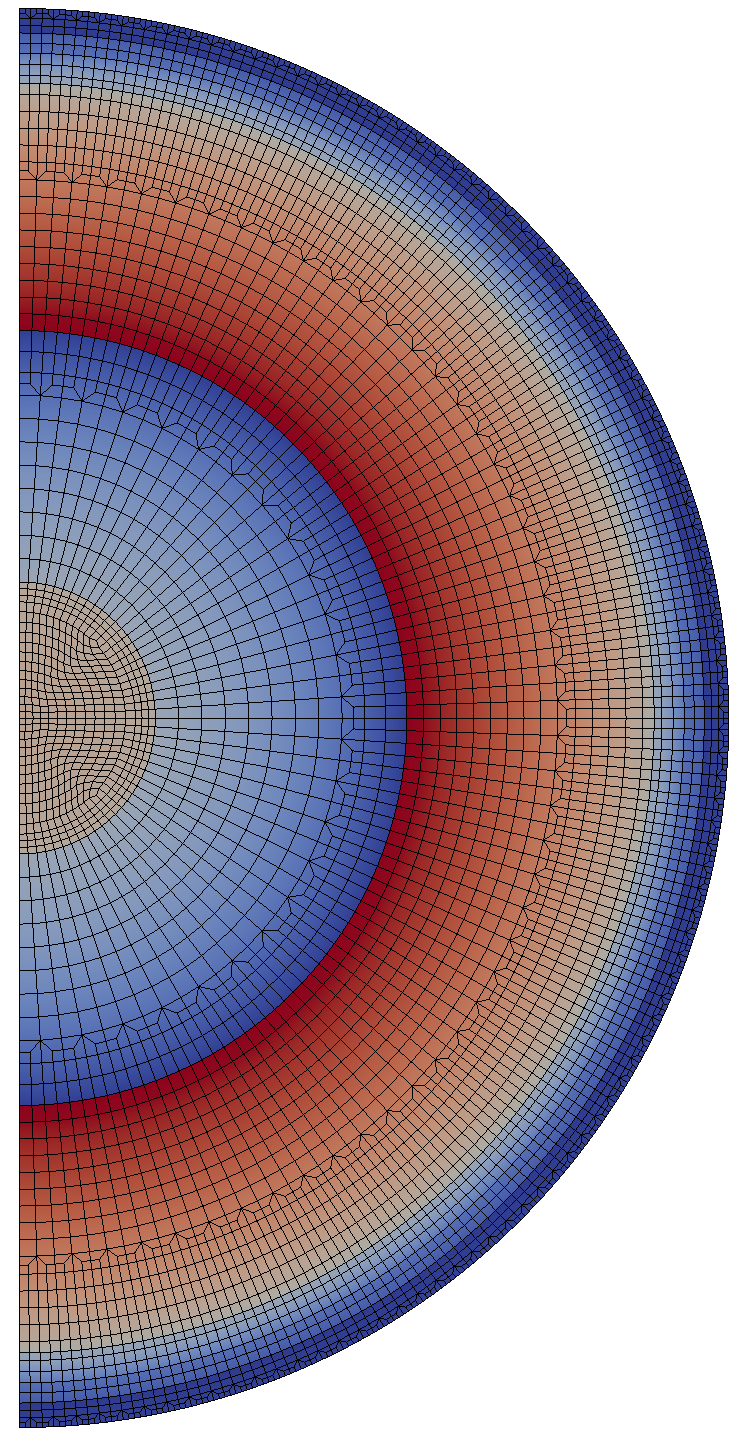
\includegraphics[width=.7\textwidth]{mesh.png}
    \end{minipage}%
\end{center}

\newpage


\subsection{Software and hardware requirements}


\subsubsection{Essential requirements}

\begin{description}
    \item[Operating system] The software should run on any UNIX-like operating system and has
          been tested on Linux (Debian, Ubuntu, SuSe, RedHat, Mageia, Cray et al) and MacOS X.
    \item[Compilers:] Fortran 90 compiler (tested on ifort, gfortran-4.6, portland, Cray)
    \item[Libraries:] MPI, NetCDF (optional), fftw (optional)
    \item[Systems:] Unix-based OS on desktop scale (tested on Linux and MacOS)\\ and HPC scale (tested on Cray XT4, XE6 and XK7, HECToR (UK National Supercomputing Service), SuperMUC (Leibniz-Rechenzentrum, Garching), Pacman (Arctic Region Supercomputing Center).
    \item[Tools:] tcshell, perl
\end{description}\vspace*{0.3cm}

\textbf{Useful tools}

\begin{description}
    \item[ObsPy:] Needed for the automated tests. Follow the instructions for your system
          on \url{http://www.obspy.org}.
    \item[Paraview:] Can be used to check meshes and watch wavefield movies.
    \item[Google Earth:] Can be used for a quick overview on seismograms at the locations
          of the receivers.
    \item[gnuplot:] Used to make quick overview plots
    \item[matlab:] Used for plotting record section (script included)
\end{description}


\subsubsection{NetCDF}
\label{sssec:netcdf}

AxiSEM allows to output larger datasets, especially wavefields in the NetCDF format. \\
Unfortunately, the installation of the NetCDF libraries may still be cumbersome; below we
list some limited support for installing NetCDF..

\begin{description}
    \item[HPC systems:] The libraries should be provided by the system. Use the
          recommended settings.
    \item[Ubuntu 12.10 and newer, Debian Wheezy and newer]: The code is working with the NetCDF libraries delivered
          with the system (for gfortran). They can be installed by \\
          \verb|sudo apt-get install libnetcdff5|
    \item[Ubuntu 12.04 and older; MacOS]: The libraries delivered with Ubuntu 12.04 and
          earlier do not seem to work reliably. We therefore generally recommend to
          compile the NetCDF libraries from source. This can be done with the script
          \textit{make\_netcdf.sh} in the \verb|SOLVER/UTILS| directory. It downloads
          current versions of the zlib, hdf5 and netcdf4 libraries from
          \url{http://www.unidata.ucar.edu}, compiles them and runs the included tests. By
          default, the new libraries are installed in \verb|$(HOME)/local|. In the first
          lines of the script, specify your compiler (has to be the same as the one you
          are using for AxiSEM). The script should be run from a scratch directory like
          \verb|/tmp|:\\
          \verb|cd /tmp|\\
          \verb|$AXISEM_DIRECTORY/SOLVER/UTILS/make_netcdf.sh|\\
          Especially the HDF5 compilation can half an hour and will produce tons of warnings. They can be
          ignored, as long as the tests pass. If one of the tests should fail, the reason
          is most likely a wrong compiler configuration. We can offer only very limited
          support for the compilation of the libraries.
    \item[Windows]: While we never tested it, installation of NetCDF on Windows should be
          possible: \url{http://www.unidata.ucar.edu/software/netcdf/docs/faq.html#windows_netcdf4_2}
\end{description}


\subsection{Preparation of a Debian/Ubuntu Linux system}
To prepare a fresh Debian-based Linux system, the absolutely necessary packages can be installed with:\\ \\
 \verb|sudo apt-get install gfortran build-essential tcsh openmpi-bin libopenmpi-dev|\\ \\
The processing and visualization tools can be installed with:\\ \\
 \verb|sudo apt-get install paraview gnuplot|

\newpage

\section{Running the code}

\subsection{Quick start}

This is the step-by-step, blackbox procedure, i.e. running a workflow from raw source code
to analyzing seismograms and wavefield movies upon pre-set parameters. It assumes your
system fulfils all requirements mentioned above.\\

\begin{center}
    \fbox{\parbox{0.65\textwidth}{
    The default simulation parameters are:
    \begin{description}
        \item[PREM] velocity model (isotropic, anelastic, continental crust)
        \item[50 s] dominant period of the mesh
        \item[2 CPUs] used for the SOLVER
        \item[1800s] seismogram length
        \item[Vertical dipole] source
        \item[100 km] source depth
    \end{description}
    } }
\end{center}

\noindent Start from within the {\tt AXISEM} directory:

\begin{enumerate}
    \item \verb|./copytemplates.csh| $\Rightarrow$ creates various input files from templates
    \item Check file \verb|make_axisem.macros| whether the compiler settings fit your
          system.
    \item \verb|cd MESHER|
    \item Check file {\tt inparam\_mesh} for background model, period of simulation and
          number of CPUs \\
          Default is \textit{PREM}, \textit{50 s} and \textit{2 CPUs} to be running within a
          few minutes on a modern PC.
    \item \verb|./submit.csh| $\Rightarrow$ Check file {\tt OUTPUT}.
    \item Wait for ``{\tt ....DONE WITH MESHER}'' to appear in {\tt OUTPUT}.
    \item move mesh files to \verb|../SOLVER/MESHES/| directory and give it a name
          \verb|./movemesh.csh PREM_50s|
    \item \verb|cd ../SOLVER|
    \item In \verb|inparam_basic| set the value for \verb|MESHNAME| to the meshname from
          above (here: \verb|PREM_50s|)
    \item \verb|./submit.csh PREM_mrr_50s_gauss_1800s|  $\Rightarrow$ compiles and runs
          the code
    \item \verb|cd PREM_mrr_50s_gauss_1800s| $\Rightarrow$ go to the run directory.
    \item Wait for ``\verb|PROGRAM axisem FINISHED|'' to appear in
          \verb|OUTPUT_PREM_mrr_50s_gauss_1800s| \\
          (use \verb|tail -f OUTPUT_PREM_mrr_50s_gauss_1800s|).
    \item \verb|./post_processing.csh|
    \item \verb|cd Data_Postprocessing|
    \item \verb|googleearth|, open {\tt googleearth\_src\_rec\_processed.kml}, click
            earthquake (info), receivers (seismograms).
    \item {\tt matlab}, run {\tt plot\_record\_section.m}, plotting all components
            of displacement seismograms.

\end{enumerate}
If the Solver is re-run with different parameters but the same mesh, you may start at step 9.
To change model, frequency or number of CPUs, repeat steps 3. to 7. and select the new
mesh in \verb|SOLVER/inparam_basic|. \\
The solver input can be changed in \verb|inparam_basic| between 8. and 9.,
changing post-processing input between 11. and 12. Using a new mesh requires
recompilation of the solver (done automatically in step 9.). If post
processing parameters are changed, also change the post processing directory or
delete the old one.


\subsection{MESHER - generate a Mesh}

\begin{enumerate}
    \item Open a terminal, go to the \ttilde\verb|MESHER| folder and open
    the \verb|inparam_mesh| file with your favourite editor:
    %
    \begin{verbatim}
    $ cd MESHER
    $ vi inparam_mesh
    \end{verbatim}
    %
    The parameters should be readily set, but you might want to double check and verify:
    %
    \begin{verbatim}
    BACKGROUND_MODEL    'prem_iso'
    DOMINANT_PERIOD     50.0
    NTHETA_SLICES       2
    NRADIAL_SLICES      1
    WRITE_VTK           true
    COARSENING_LAYERS   3
    \end{verbatim}
    %
    The file should be self-explanatory. NB: Models without crust ('light') allow for a
    larger time step and hence run a lot faster. \\
    WARNING: Only write vtk files if the dominant period is rather large, i.e. above 10 or
    20s, as these files become exceedingly large.

    \item Run the mesher, and watch the progress:
    %
    \begin{verbatim}
    $ ./submit.csh
    $ tail -f OUTPUT
    \end{verbatim}
    %
    The meshing should be really fast (i.e. on the order of seconds) for the chosen parameters. Wait for
    \verb|....DONE WITH MESHER !| to appear.

    \item Take a look at the mesh with paraview
    \begin{verbatim}
    $ paraview
    \end{verbatim}
    %
    Open one of the vtk files in the subfolder \verb|Diags|, e.g.\
    \verb|mesh_vp.vtk| and click apply in the properties panel on the left (you
    might get an OpenGL Error on the virtual box, which you can ignore). To see
    the mesh, change the representation from 'surface' to 'surface with edges'
    (On some host systems, the dropdown menu seems to be messed up, in that
    case go to the 'Display' context in the 'Properties' panel on the left. If
    the plot appears all yellow, click on play).  You can open other vtk files
    to look at other properties of the model and the mesh. You might need to
    rescale the color range by clicking on the left-right arrow symbol in the
    top left.

    \begin{center}
    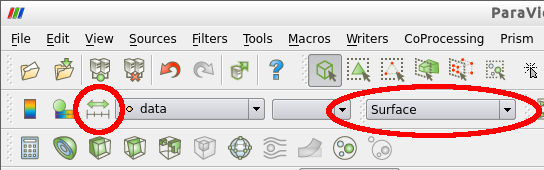
\includegraphics[height=30mm]{paraview.png}
    \hspace{5mm}
    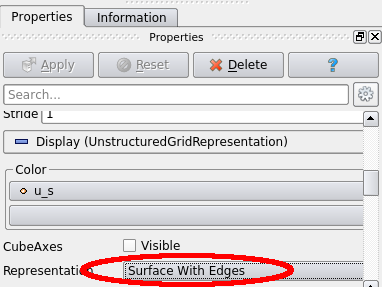
\includegraphics[height=30mm]{paraview3.png}
    \end{center}

    \item Move the mesh to the solver directory and give it a meaningful name:
    \begin{verbatim}
    $ ./movemesh.csh PREM_50s
    \end{verbatim}

\end{enumerate}

\newpage
\subsection{SOLVER - solve the elastic wave equation}

\begin{enumerate}
    \item Go to the \ttilde\verb|SOLVER| folder and open the
    \verb|inparam_basic| file with your favourite editor:
    %
    \begin{verbatim}
    $ cd ../SOLVER
    $ vi inparam_basic
    \end{verbatim}
    %
    Set these parameters:
    %
    \begin{verbatim}
    SIMULATION_TYPE     single
    SEISMOGRAM_LENGTH   1800.
    RECFILE_TYPE        stations
    MESHNAME            PREM_50s
    ATTENUATION         true
    SAVE_SNAPSHOTS      true
    \end{verbatim}
    %
    WARNING: Only save snapshots if the mesh is rather low resolution,
    e.g. above 20s as these files become exceedingly large. You may
    alternatively opt to only plot a fraction of the 2D domain which
    can be set in \verb|inparam_advanced|.

    \item First, we are taking a look at a basic sourcetype: a vertical dipole, which has
    a monopole radiation pattern. This is set by \verb|SIMULATION_TYPE single| and defined
    in the \verb|inparam_source| file. Run the solver, giving the run a meaningful name:
    %
    \begin{verbatim}
    $ ./submit.csh PREM_mrr_50s_gauss_1800s
    \end{verbatim}
    %
    This command compiles the code if needed and starts the simulation. You can observe
    the progress in the outputfile:
    %
    \begin{verbatim}
    $ cd PREM_mrr_50s_gauss_1800s
    $ tail -f OUTPUT_PREM_mrr_50s_gauss_1800s
    \end{verbatim}
    %
    Once the run is finished, take a look at the wavefield with \verb|paraview|: open
    the \verb|PREM_mrr_50s_gauss_1800s/| \verb|Data/xdmf_xml_0000.xdmf|
    file and click apply. Go to the last snapshot and rescale the color range,
    then click on play to see the wave propagate.  You can also choose
    different components of the wavefield or the absolute value.  For paraview
    experienced users: choose absolute value and a logarithmic colorscale to
    see all wave types at once (e.g.\ 'black body radiation' looks nice).

    \begin{center}
    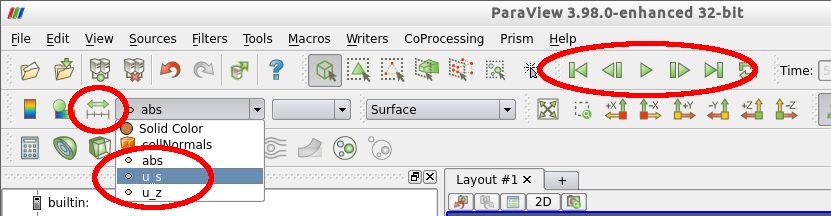
\includegraphics[width=110mm]{paraview2.png} \hspace{5mm}
%    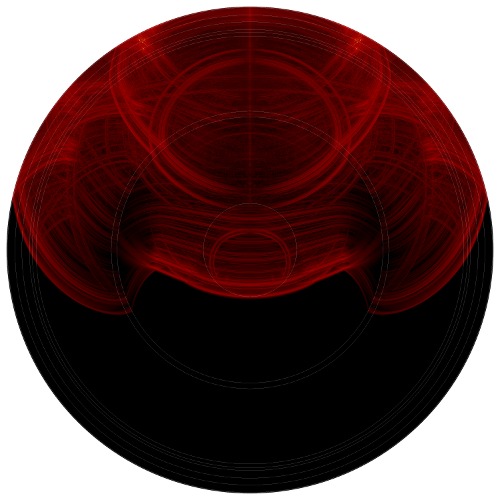
\includegraphics[width=40mm]{0600.png}
    \end{center}

    \item Now simulate seismograms for a full moment tensor source: the source is defined
    in the \verb|CMTSOLUTION| file and the one referred to as 'event-1' in the later tasks.
    Stations are defined in the \verb|STATIONS| file. Go back to the \verb|SOLVER|
    directory and change the \verb|inparam_basic| file such that:
    %
    \begin{verbatim}
    SIMULATION_TYPE     moment
    SAVE_SNAPSHOTS      false
    \end{verbatim}
    %
    Run the solver, giving the run a meaningful name:
    %
    \begin{verbatim}
    $ ./submit.csh prem_50s_event1
    \end{verbatim}
    %
    This command compiles the code if needed and starts four simulations at once, each
    simulating a basic source type (two monopoles, a dipole and a quadrupole, for details
    see \textit{Nissen-Meyer et al., 2007}). You can observe the progress in the outputfiles in
    each job's subdirectory
    %
    \begin{verbatim}
    $ cd prem_50s_event1
    $ tail -f MZZ/OUTPUT_MZZ
    \end{verbatim}
    %
    Once all the jobs are done (check with \verb|htop|), you can proceed with
    postprocessing.

\end{enumerate}


\subsection{POSTPROCESSING - rotate and sum seismograms and wavefields}

Postprocessing is a key feature of AxiSEM: the source mechanism and source time function
can be modified without redoing the more expensive simulation.

\begin{enumerate}
    \item For the previous simulation, the contribution of the elemental sources needs
    to be summed up to get seismograms for a full moment tensor source. In the
    main rundirectory (\verb|prem_50s_event1|) open the file
    \verb|param_postprocessing|. It should contain these settings (auto generated by the
    solver):
    %
    \begin{verbatim}
    REC_COMP_SYS    enz
    CONV_PERIOD     0.
    CONV_STF        gauss_0
    \end{verbatim}
    %
    The source mechanism (depth and location cannot be changed in postprocessing) is read
    from the \verb|CMTSOLUTION| file in the same directory. Start the postprocessing:
    %
    \begin{verbatim}
    $ ./postprocessing.csh
    \end{verbatim}
    %
    The resulting seismograms and plots can be found in the directory
    \verb|Data_Postprocessing|. Seismograms can be viewed with your favorite image viewer,
    e.g.\ \verb|eog|:
    %
    \begin{verbatim}
    $ cd Data_Postprocessing/GRAPHICS
    $ eog <filename.gif>
    \end{verbatim}
    %
    For a nice overview, you can use \verb|google-earth| (might not run on all computers
    and depends on internet connection). Open the \verb|googleearth_src_rec_seis.kml| file
    in the \verb|Data_Postprocessing/| directory (double check the exact path,
    google-earth might have something older from history which is quite confusing).
    You should now see the earthquake and the receivers in the places menu on the left.

    \begin{center}
    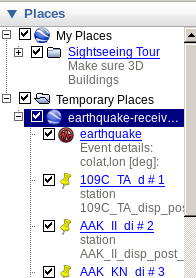
\includegraphics[height=70mm]{google-earth.png}
    \hspace{5mm}
    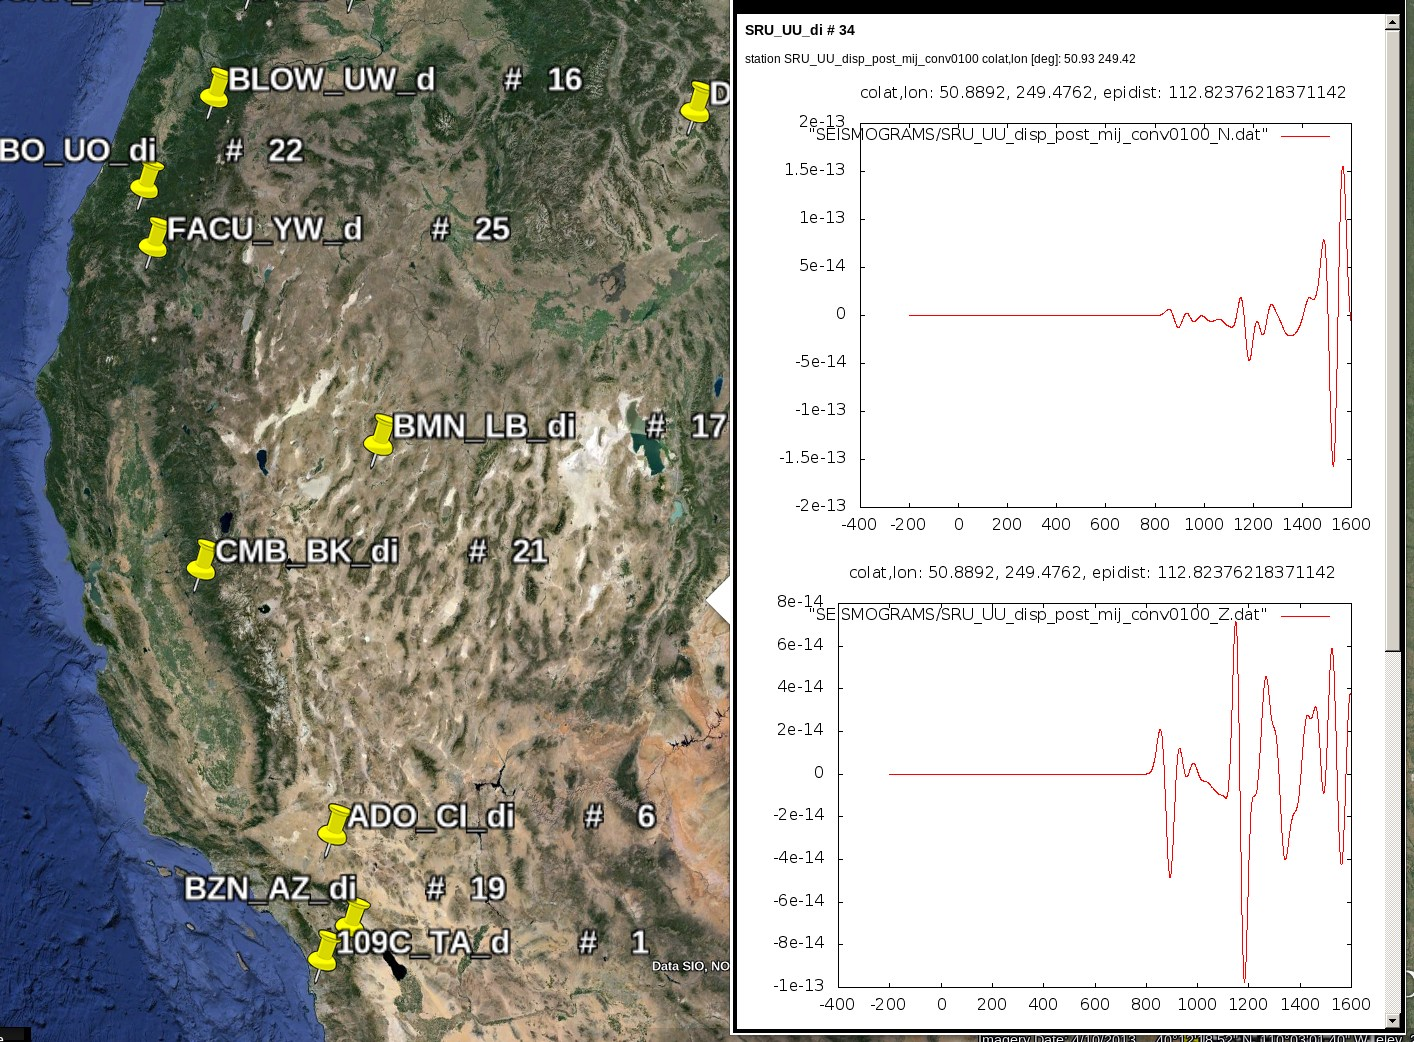
\includegraphics[height=70mm]{google-earth2.jpg}
    \end{center}

    Click on the stations or source to see more...

\end{enumerate}

\subsection{Computational aspects}

Running in a 2D computational domain, the code is (obviously) significantly faster
than comparable 3D methods.

\begin{center}
    %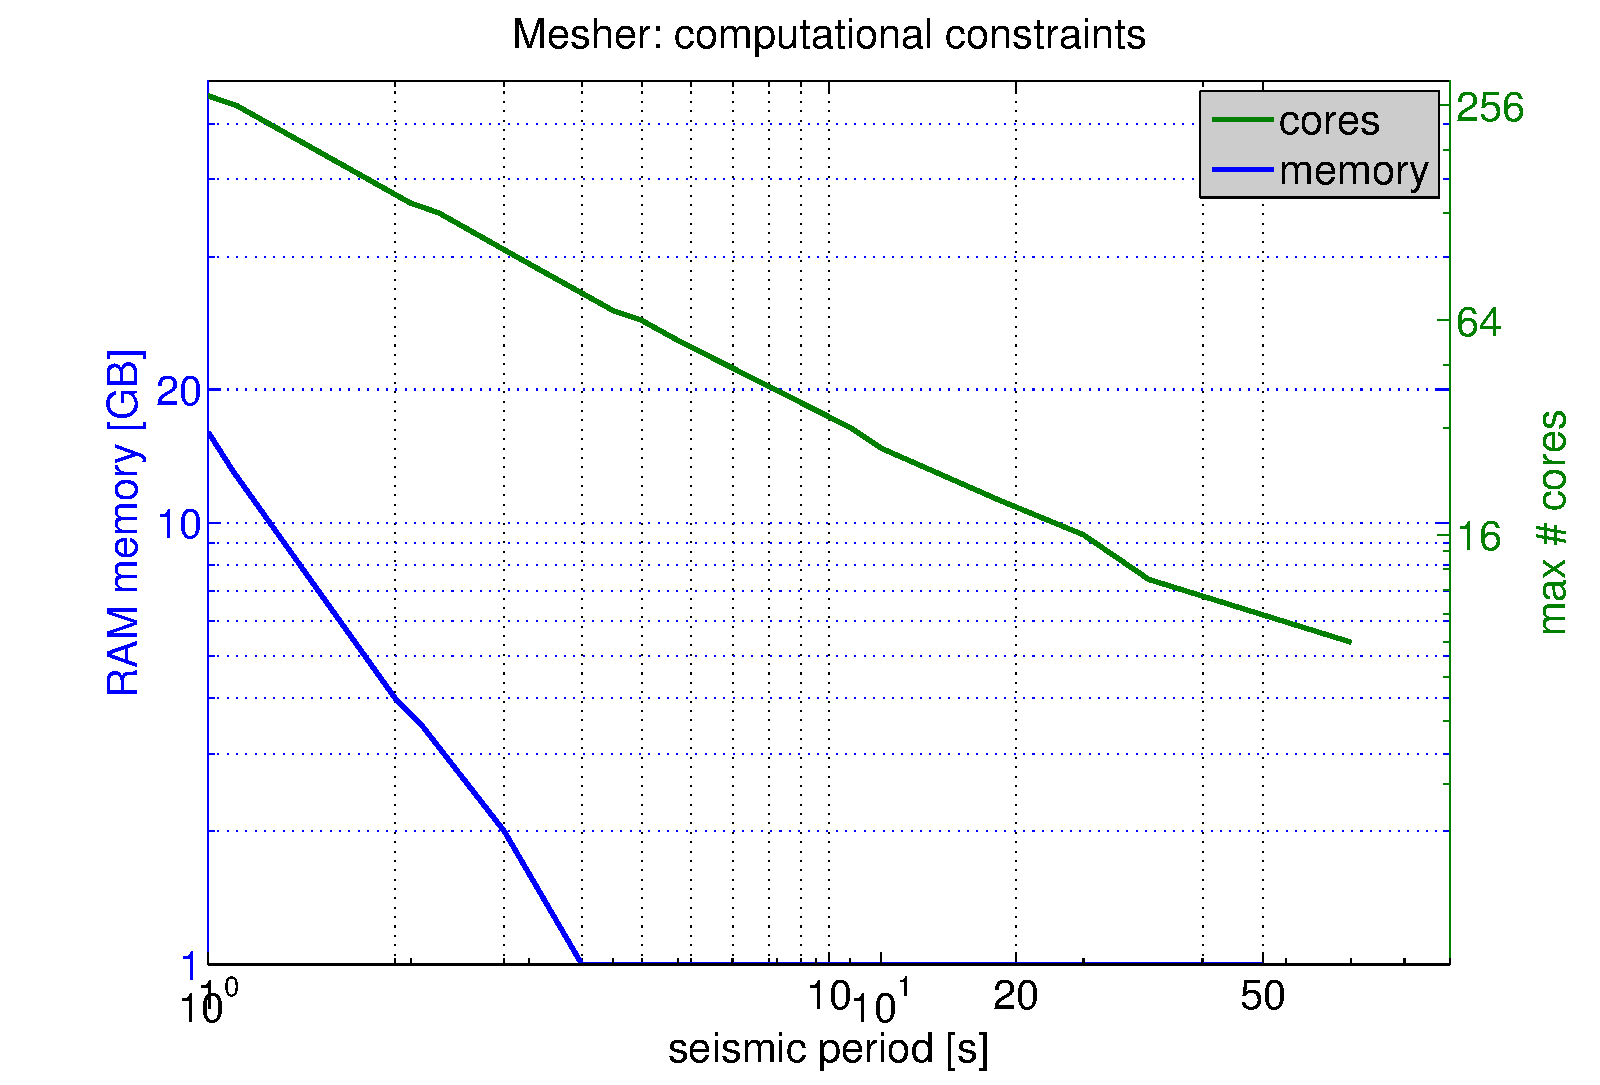
\includegraphics[height=50mm]{mesher_comp_cost.pdf}
    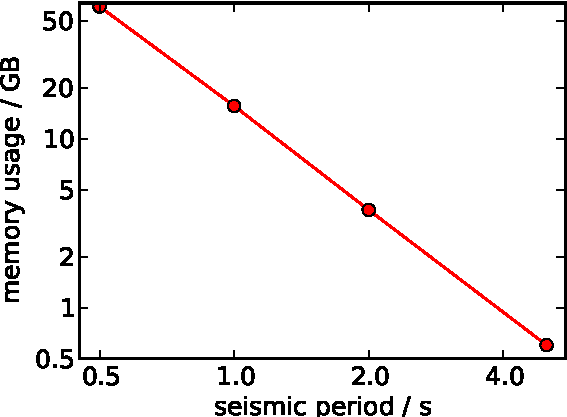
\includegraphics[height=50mm]{memory_usage_new.pdf}
    \hspace{5mm}
    %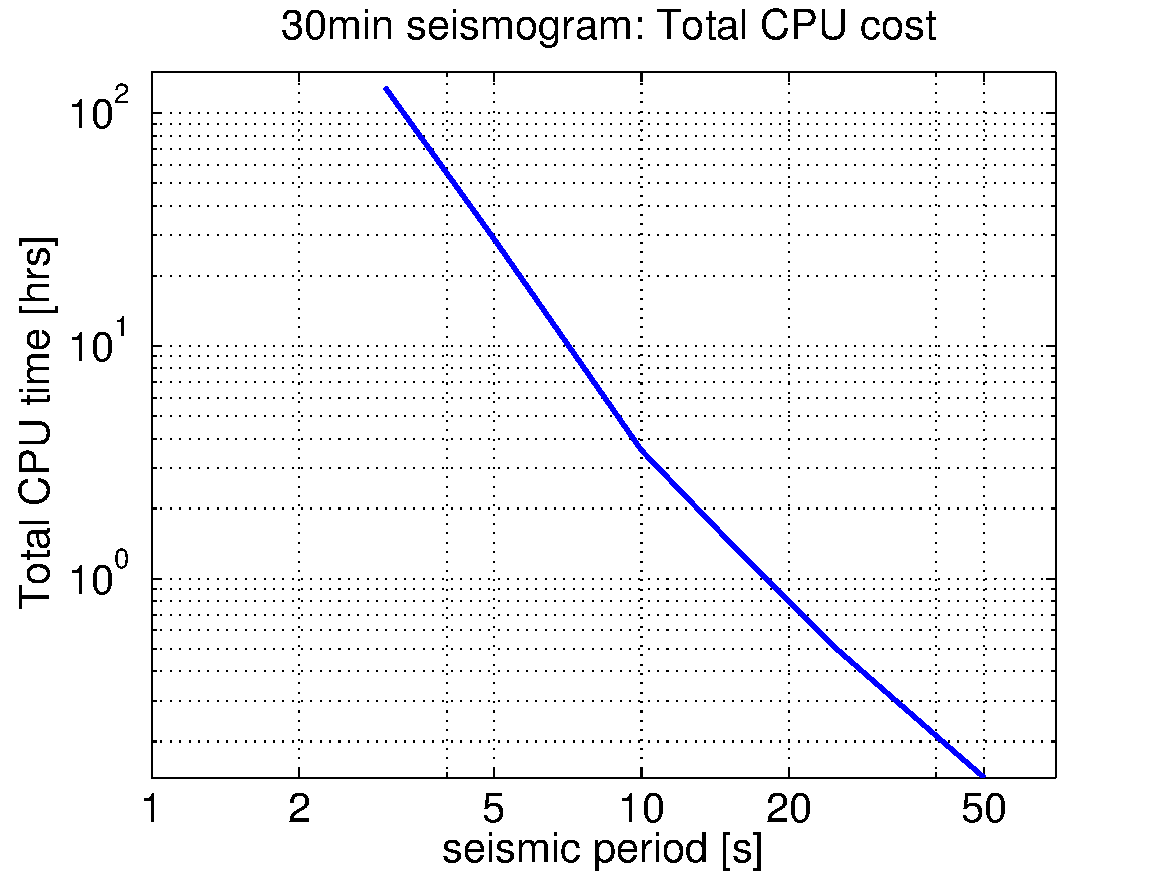
\includegraphics[height=50mm]{solver_totalcpu.pdf}
    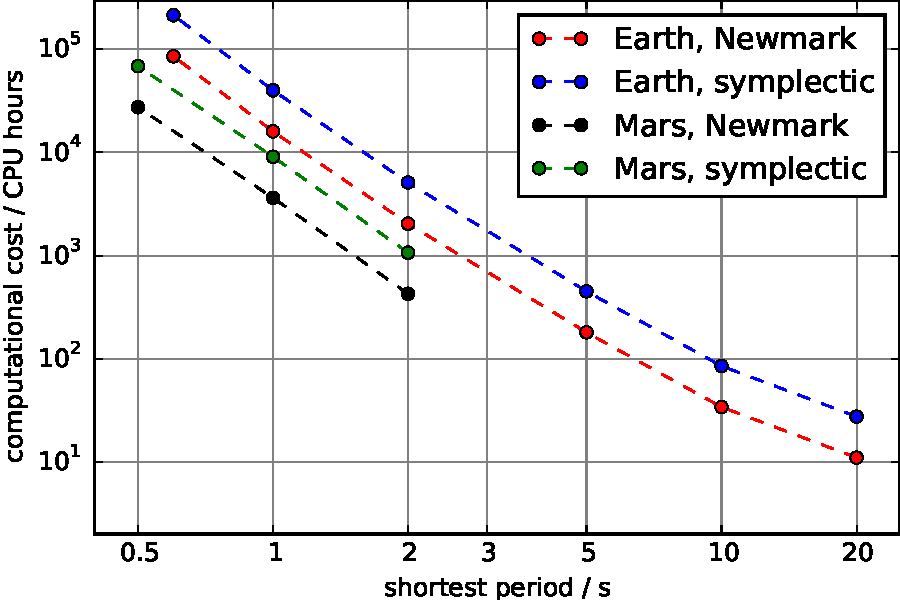
\includegraphics[height=50mm]{db_generation_cost.pdf}
\end{center}

On the left, you may deduct the mesher's RAM occupation as a function of frequency. Going
towards very high resolution (around and above 1Hz), you will need a rather fat node (>
16GB RAM) for the (shared memory) meshing.
On the right, we depict the computational cost
associated with the solver to compute seismograms of one hour length for Earth and Mars
and for the second order Newmark as well as the fourth order symplectic time scheme. The
relation between seismic period and CPU-hours is an approximate proxy to estimate how many
cores and wall-clock time is optimal for your infrastructure. Scaling of CPU hours is
approximately to the third power of the maximum frequency. As a rule of thumb, using the
symplectic scheme is advisable when propagating waves for more than 100 wavelengths.

\begin{center}
    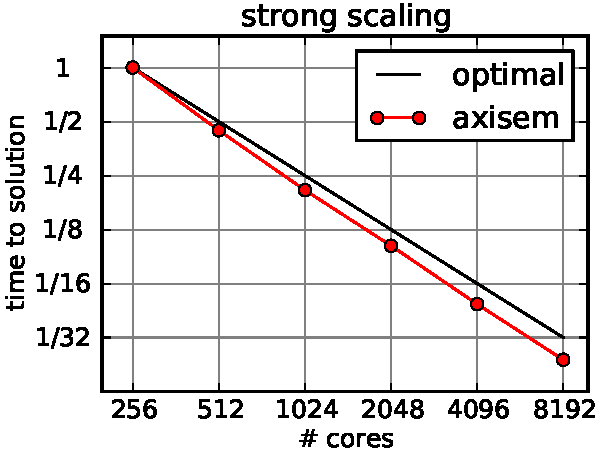
\includegraphics[height=50mm]{COMPUTATIONAL_COST/strong_scaling_new.pdf}
    \hspace{5mm}
    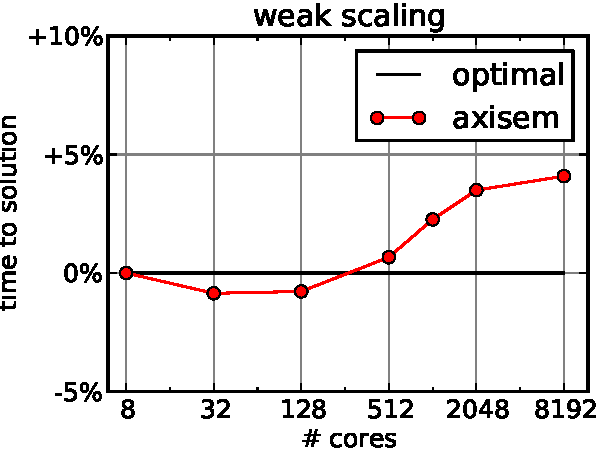
\includegraphics[height=50mm]{COMPUTATIONAL_COST/weak_scaling_new.pdf}
\end{center}

Scalability plots from test runs on a Cray machine at CSCS, Switzerland. The left shows
strong scaling (fixed global problem size), the right plot weak scaling (fixed problem
size per CPU).


\section{Typical use cases}

\subsection{Change source type}

\verb|SOLVER/inparam_source|, \verb|SOLVER/CMTSOLUTION| and \verb|SOLVER/inparam_basic|.
AxiSEM has three principal modes, which are selected by the value \verb|SIMULATION_TYPE| in
\verb|SOLVER/inparam_basic|.

\begin{enumerate}
\item \verb|SIMULATION_TYPE single|:\\ The Solver simulates one basic source, which can be
      one of the following:\\
      \begin{center}
        \begin{tabular}{|l|cccc|} \hline
         monopoles:   & $M_{rr}$ & explosion  & $M_{\theta\theta}+M_{\phi\phi}$  & $P_r$ \\
         dipoles:     & $M_{\theta r}$ & $M_{\phi r}$        & $P_{\theta}$ & $P_{\phi}$\\
         quadrupoles: & $M_{\theta \phi}$ & $M_{\theta\theta}-M_{\phi\phi}$ & & \\\hline
        \end{tabular}
      \end{center}
      where $M_{ii}$ are moment tensor sources with the mentioned components of $M$ set to
      one and the others to zero, $P_i$ is the same for single forces.\\ Choose the source
      type and set the source depth and amplitude in \verb|SOLVER/inparam_source|.

\item \verb|SIMULATION_TYPE moment|:\\
      The submit.csh script starts four separate simulations for the basic types $M_{rr}$,
      $M_{\theta\theta}+M_{\phi\phi}$, $M_{\theta r}$, $M_{\theta \phi}$. You have to run
      the postprocessing script after the simulation to sum them up correctly. \\ Before
      the simulation, set the source depth and the moment tensor in
      \verb|SOLVER/CMTSOLUTION|. \\Run \verb|postprocessing.csh| in the simulation
      directory afterwards. You can run postprocessing for different moment tensors on the
      same simulation, but not for different depths (since the forward simulation depends
      on the depth).  The \verb|CMTSOLUTION| file is a standard format and can be
      downloaded from many sites in the web, including
      \url{http://www.globalcmt.org/CMTsearch.html}

\item \verb|SIMULATION_TYPE force|:\\
      The submit.csh script starts two separate simulations for the basic types $P_r$ and
      $P_\theta$. This mode is used to compute the databases for instaseis. Note, that the
      postprocessing does not handle these runs yet appropriately.
\end{enumerate}

\subsection{Change station locations}

\verb|SOLVER/STATIONS| or \verb|SOLVER/receivers.dat|, depending on
\verb|SOLVER/inparam_basic|, parameter \verb|RECFILE_TYPE|\\

\verb|SOLVER/STATIONS|: Similar to \textit{SPECFEM3D Globe}, an ASCII file with six
columns, which are: station name, network name, latitude, longitude, elevation, depth
(n.b: AxiSEM puts all receivers to the surface, the last two rows are ignored).

\begin{verbatim}
 RAYN   GD  23.52   45.50  0.0  0.0
 PALK   GD   7.27   80.70  0.0  0.0
 MAJO   GD  36.54  138.21  0.0  0.0
 ERM    GD  42.02  143.16  0.0  0.0
\end{verbatim}

The station names are used by post\_processing to assign names to the seismogram files.\\
\verb|SOLVER/receivers.dat|: Plain ASCII file with number of receivers in the first line
and then nrec lines with colatitude and longitude.

\begin{verbatim}
 7
0.0 0.0
30.0 0.0
60.0 0.0
90.0 0.0
120.0 0.0
150.0 0.0
180.0 0.0
\end{verbatim}


\subsection{Change background model}

\verb|MESHER/inparam_mesh|, parameter \verb|BACKGROUND_MODEL|:\\
afterwards the steps from 5 have to be rerun. Supported models are

\begin{verbatim}
# prem_iso:               Isotropic continental PREM model
# prem_iso_solid:         like 'prem_iso', replace fluid outer core with vs=vp/sqrt(3)
# prem_iso_onecrust:      like 'prem_iso' but extend lower crust to surface
# prem_iso_light:         like 'prem_iso' but with mantle material extended to surface
# prem_iso_solid_light:   like 'prem_light', but in fluid outer core vs=vp/sqrt(3)
#
# prem_ani:               Anisotropic continental PREM model (actual PREM)
# prem_ani_onecrust:      like 'prem_ani' but extend lower crust to surface
# prem_ani_light:         like 'prem_ani' but with mantle material extended to surface
#
# ak135                   AK135 (Isotropic, PREM attenuation)
# ak135f                  AK135 (Isotropic, own attenuation)
# iasp91:                 Isotropic IASP91 model with PREM density and attenuation
# external:               Layered external model, give file name in EXT_MODEL, the
#                         inner core needs to be big enough, check VTK output.
\end{verbatim}


\subsection{Use external 1D velocity model}

\verb|MESHER/inparam_mesh|, change parameter \verb|BACKGROUND_MODEL| to \verb|external|
and \verb|EXT_MODEL| to the filename of your model. The model should be stored in a file
of the following form:

\begin{verbatim}
ANELASTIC       T
ANISOTROPIC     T
UNITS           m
COLUMNS     radius    rho    vpv    vsv    qka    qmu  vph   vsh   eta
            6371000.  2600.  5800.  3200.  57827. 600. 5800. 3200. 1.00000
            6356000.  2600.  5800.  3200.  57827. 600. 5800. 3200. 1.00000
#          Discontinuity   1, depth:      15.00 km
            6356000.  2900.  6800.  3900.  57827. 600. 6800. 3900. 1.00000
            6346600.  2900.  6800.  3900.  57827. 600. 6800. 3900. 1.00000
#          Discontinuity   2, depth:      24.40 km
            6346600.  3380.  8190.  4396.  57827. 600. 8190. 4611. 0.90039
            6341600.  3380.  8186.  4397.  57827. 600. 8186. 4607. 0.90233
            6336600.  3379.  8183.  4398.  57827. 600. 8183. 4602. 0.90428
            6331600.  3379.  8179.  4399.  57827. 600. 8179. 4598. 0.90622

\end{verbatim}

In the header, four keywords are mandatory to describe the following model:
\begin{itemize}
 \item \verb|ANELASTIC|: Is the model anelastic (viscoelastic) or not?
 \item \verb|ANISOTROPIC|: Is the model anisotropic or not?
 \item \verb|UNITS|: Are the units in this file given in \textit{SI}-units? Allowed values:
       \begin{itemize}
        \item \verb|m| \textit{SI}-units: (m, m/s, kg/m$^3$)
        \item \verb|km| km, km/s, g/cm$^3$. These units are often used because the values are between 1 and 10.
       \end{itemize}
 \item \verb|COLUMNS|: Describe the column order in the file. Necessary values:
  \begin{itemize}
  \item For an elastic, isotropic model:
    \begin{itemize}
    \item \verb|radius|/\verb|depth| (radius or depth of the layer. Allows to define the position of the layers in radius (beginning from the center) or depth (beginning from the surface)
    \item \verb|rho| ($\rho$, density)
    \item \verb|vpv| ($\alpha$, vertical P-velocity)
    \item \verb|vsv| ($\beta$, vertical S-velocity)
    \end{itemize}
  \item For an anelastic model additionally:
    \begin{itemize}
    \item \verb|qka| ($Q_{\kappa}$)
    \item \verb|qmu| ($Q_{\mu}$)
    \end{itemize}
  \item For an anisotropic model additionally:
    \begin{itemize}
    \item \verb|vph| (horizontal P-velocity)
    \item \verb|vsh| (horizontal S-velocity)
    \item \verb|eta| (anisotropic parameter $\eta$)
    \end{itemize}
  \end{itemize}
\end{itemize}

This header is followed by an arbritrary number of lines with velocity layers, where \verb|#| marks comment lines. The header variables \verb|UNITS| and \verb|COLUMNS| allow to customize the structure of these lines, which should facilitate the import of external models from other programs.

First order discontinuities are enforced by double layers with the same radius (see layers 2/3 and 4/5
in the example) and are honoured by the MESHER.

For an example file, select one of the internal models in \verb|MESHER/inparam_mesh|, enable the option \verb|WRITE_1DMODEL| and run the MESHER. It will write a valid input file of the selected model into \verb|MESHER/Diags/1dmodel_axisem.bm|. Modify this file according to your needs.

The overall radius of the body is given by the radius of the outermost layer and can take
any reasonable value (Read: Planets, moons and tennis balls can be simulated, single electrons probably not).

\subsection{Change number of CPUs}

\verb|MESHER/inparam_mesh|, parameter \verb|NTHETA_SLICES| and \verb|NRADIAL_SLICES|: \\
The number of CPUs used is the product of the two parameters. \\
\verb|NTHETA_SLICES| needs to be 1, 2, 4 or a multiple of 4. To get a suggestion for
optimal decomposition, run the Mesher with \verb|ONLY_SUGGEST_NTHETA true| and check the
OUTPUT file.\\
\verb|NRADIAL_SLICES| should be on the order of 8, larger numbers work for very high
frequencies. It can be left at 1 for \verb|NTHETA_SLICES|<64 CPUs, but should be increased
then to reduce MPI communication. To ensure scaling, each processor should have at least
about 500 elements.\\
N.B: This value is for ONE simulation. To calculate the wavefield of a full moment tensor,
4 parallel simulations have to be run and the number of necessary CPUs is
\verb|NTHETA_SLICES|* \verb|NRADIAL_SLICES|*4.


\subsection{Change the maximum frequency of the simulation}
\verb|MESHER/inparam_mesh|, parameter \verb|DOMINANT_PERIOD|: \\
As a rule of thumb: Simulations with \verb|DOMINANT_PERIOD|>10s can be run with 2 or 4
CPUs on a modern workstation and cost around 1 CPUh.


\subsection{Calculate the response to a full moment tensor solution}
\verb|SOLVER/inparam_basic|, change parameter \verb|SIMULATION_TYPE| to \verb|moment|:\\
The moment tensor, depth and location of the source must be set in the file
\verb|CMTSOLUTION|. The submit.csh script starts four separate runs in parallel, the
postprocessing script sums the results to get correct seismograms.


\subsection{Change source time function}
\verb|SOLVER/inparam_advanced|, change parameter \verb|SOURCE_FUNCTION||:\\
AxiSEM generally calculates displacement seismograms. The source time function selected
here is equivalent to the moment function $m(t)$. Note that to calculate seismograms
similar to those of an earthquake (i.e. with a persistent displacement at the source), the
setting \verb|errorf| has to be used. Note that that is different to the literature that
usually defines the source time function as the moment rate function $\dot{m}(t)$.
However, it is consistent with SpecFEM.\\
To create seismograms with a flat, zero-phased source spectrum, use the setting
\verb|dirac_0|. Seismograms calculated with this setting can be convolved with other
source functions in AxiSEM postprocessing or manually with a program of your choice.\\
However, note that seismograms or wavefields calculated with a \verb|dirac_0| STF will
contain numerical noise. Therefore, visualization and wavefield plotting should be done
using \verb|errorf| or one of the Gaussian STFs.


\subsection{Change seismogram length or sampling rate}
\verb|SOLVER/inparam_basic|, change parameter \verb|SEISMOGRAM_LENGTH|:\\
Default value is 1800~s, although the exact length is rounded to the next multiple of the
simulation time step. There is no maximum limit, AxiSEM has been run for 400000s (5 days)
to compare amplitude spectra with a normal modes summation (Nissen-Meyer et al, 2014).\\
\verb|SOLVER/inparam_advanced|, change parameter \verb|SAMPLING_RATE|:\\
By default, the sampling rate is set to the time step length of the simulation. We
strongly recommend to leave it as such to avoid aliasing. The resampling can better be
done with \textit{ObsPy} or another tool that supports filtering.

\subsection{Output wavefields in netcdf format needed for \textit{Instaseis}}

\begin{itemize}
    \item Compile with netcdf (see section~\ref{sssec:netcdf} for hints on the
    installation): in \verb|make_axisem.macros| set \verb|USE_NETCDF| to \verb|true|
    and if netcdf is not in your \verb|PATH|, also set \verb|NETCDF_PATH| to the location
    of your netcdf installation. If you have netcdf compiled with MPI and run on a
    supercomputer, using \verb|USE_PARALLEL_NETCDF true| might be beneficial for short
    period runs.
    \item In \verb|SOLVER/inparam_advanced| set \verb|USE_NETCDF| to \verb|true| to
    use netcdf output in the solver
    \item In \verb|SOLVER/inparam_advanced| set \verb|DATA_DIR| to some location where you
    have enough free space and in case you use parallel IO this should be on a parallel
    file system
    \item further settings in \verb|SOLVER/inparam_advanced| to generate a full database,
    that is all epicentral distances and source down to 700km and using the fourth order
    spatial scheme:

\begin{verbatim}
SOURCE_FUNCTION     gauss_0

KERNEL_WAVEFIELDS   true

KERNEL_DUMPTYPE     displ_only
KERNEL_SPP          4
KERNEL_SOURCE       igno

KERNEL_COLAT_MIN    0.
KERNEL_COLAT_MAX    180.

KERNEL_RMIN         5671.
KERNEL_RMAX         7000.
\end{verbatim}

    \item in \verb|SOLVER/inparam_basic| set \verb|SIMULATION_TYPE| to \verb|force| to
    simulate both the vertical and the horizontal database. To generate just one of the
    two, set it to \verb|single| and select either \verb|thetaforce| or \verb|vertforce|
    in \\\verb|SOLVER/inparam_source|

    \item once the AxiSEM runs are finished, go to the rundirectory and run
    \verb|./fieltransform.sh| (in case of single runs just run \verb|./fieltransform|
    directly). This rechunks the wavefields in the netcdf file to optimize them for
    reading as time series instead of snapshots.

\end{itemize}


\subsection{Include lateral heterogeneities (2.5D simulation)}
\verb|SOLVER/inparam_basic|, change parameter \verb|LAT_HETEROGENEITY| to true:\\
The actual heterogeneity model is set in \verb|SOLVER/inparam_hetero|.
This functionality is currently under development and not documented. See the example
files \verb|SOLVER/inparam_hetero.TEMPLATE| for an idea of what to do.


\newpage
\section{References}

\noindent \textbf{Directly dealing with this code:}\vspace*{0.2cm}\\
When using this code, please cite one or more of these publications. \vspace*{0.2cm}\\


(1) Tarje Nissen-Meyer, M. van Driel, S. C. Stahler, K. Hosseini, S. Hempel, L. Auer,
A. Colombi, and A. Fournier (2014), \textit{AxiSEM: broadband 3-D seismic wavefields
in axisymmetric media},  Solid Earth, 5, 425-445. \\
doi:10.5194/se-5-425-2014\\

(2) Tarje Nissen-Meyer, F. A. Dahlen, A. Fournier (2007),
\textit{Spherical-earth Fr\'{e}chet sensitivity kernels},
Geophysical Journal International 168(3),1051-1066. \\
doi:10.1111/j.1365-246X.2006.03123.x                \\

(3) Tarje Nissen-Meyer, A. Fournier, F. A. Dahlen (2007),
\textit{A two-dimensional spectral-element method for
spherical-earth seismograms-I. Moment-tensor source},
Geophysical Journal International 168(3), 1067-1092. \\
doi:10.1111/j.1365-246X.2006.03121.x                 \\

(4) Tarje Nissen-Meyer, A. Fournier, F. A. Dahlen (2008),
\textit{A two-dimensional spectral-element method for
spherical-earth seismograms - II. Waves in solid-fluid media},
Geophysical Journal International, 174(3), 873-888.\\
doi:10.1111/j.1365-246X.2008.03813.x\\

(5) Tarje Nissen-Meyer (2007),
\textit{Full-wave seismic sensitivity in a spherical Earth},
Ph.D. thesis, Princeton University
(This includes refs (2)-(4) and more details.)\\

(6) Martin van Driel and Tarje Nissen-Meyer (2014),
\textit{Seismic Wave Propagation in Fully Anisotropic Axisymmetric Media},
Geophysical Journal International 199 (2), 880-893.\\
doi:10.1093/gji/ggu269.\\

(7) Martin van Driel and Tarje Nissen-Meyer (2014),
\textit{Optimized Viscoelastic Wave Propagation for Weakly Dissipative Media},
Geophysical Journal International 199 (2) 1078-1093.\\
doi:10.1093/gji/ggu314.\\

%
% (5) Jean-Paul Ampuero, Tarje Nissen-Meyer (2011),
% \textit{High-order conservative time schemes in spectral-element methods
% for seismic wave propagation.}, To be submitted to Geophys. J. Int.\\

%\noindent \textbf{NOTE:} Most important sections of these papers are in the Theory section below.\\

\noindent \textbf{Other references:}\vspace*{0.2cm}

(8) Martin van Driel, Lion Krischer, Simon Stahler, Kasra Hosseini, and Tarje Nissen-Meyer (2015),
\textit{Instaseis: Instant Global Broadband Seismograms Based on a Waveform Database},
To be submitted to Solid Earth\\

(9) Deville, M. O., Fischer, P. F., Mund, E. H. (2002),
\textit{High-Order Methods for Incompressible Fluid Flow},
Vol. 2, Cambridge monographs on Sppl. \& Comp. Math., Cambridge University Press.\\

(10) Tufo, H. M., Fischer, P. F. (2001), \textit{Fast Parallel Direct Solvers For Coarse
Grid Problems}, 61, 151-177, J. Par. and Dist. Comput.\\

(11) Bernardi, C., Dauge, M., Maday, Y. (1999), \textit{Spectral Methods for Axisymmetric
Domains}, Vol. 3, Series in Appl. Math., Gauthier-Villars, Paris.\\

(12) Chaljub, E. (2000), \textit{Mod{\'{e}}lisation num{\'{e}}rique de la
propagation d'ondes sismiques en g{\'{e}}om{\'{e}}trie sph{\'{e}}rique:
Application {\`{a}} la sismologie globale},
Ph.D. thesis, Universit{\'{e}} de Paris 7.\\

(13) Komatitsch D., Tromp, J. (2002), \textit{Spectral-element simulations of
global seismic wave propagation---I. Validation},
149, 390-412, Geophys. J. Int.


\end{document}
